\section{One's weaker self}

\begin{center}
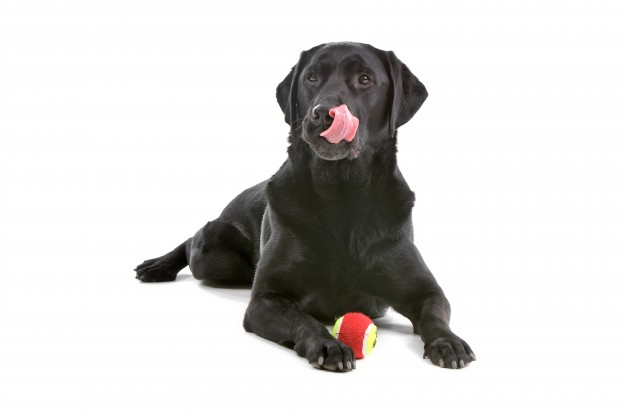
\includegraphics[width=8cm]{images/13_weak.jpg}
\end{center}

\textit{I do want to do the right thing, but how?}

We all want to do the right thing. No one wants to upset another person. Most of us believe in the actual good within each other, and so also within ourselves. Yet, we often do what we afterwards regret and feel ashamed of: We speak words that hurt others; we do not reach out our hand although we know it would be the right thing to do; we take what we want at the expense of others and find justifications why it is our right to do so.

We react in a snotty, sulky, rude, sarcastic, jealous way or like a smartass. We feel threatened and think we constantly have to defend ourselves against attacks. And we break our promises, towards others but especially towards ourselves. Just think about new year’s resolutions.

While our weaker self, this little lazy dog, runs its circles on an extremely long leash, everyone also has another part within themselves: A part which is pure, innocent, free of intention, and full of confidence and trust. So how can we evade that lazy dog and let that other part take control of the steering wheel? How can this gentle little thing outshine this loud barking dog inside of us?

The answer is simple and also, at the same time, uncomfortable:

First, we have to train that dog, so that it won't move around wildly anymore, but sit still and give us its paw. That requires some work, which in Tantric Buddhism is called "to tame the spirit". This kind of work is challenging and tedious, as the weaker self speaks in the exact same voice as the higher self does, and to be able to differentiate those two takes a lot of time.

Furthermore, we have to bring this breathtakingly beautiful, yet also very vulnerable part of us out of the protection of the darkness and make it visible.

Isn't it endangered through that? Yes, it is. Can we be hurt when we show ourselves vulnerably? Yes, we can. Will we be taken advantage of immediately and sucked empty and fall victim to sharks? Most likely not. Because that tender part of us is not totally helpless and whiny. It also doesn't blame others when something goes wrong. It is full of wonder, compassion, generosity and joy, which doesn't need a cause, and love, which doesn't ask questions. And that part is also courageous: While the weaker self (also called the "ego") turns away and mumbles "this is not my concern", the tender part (let's call it the "self") does the right thing instead: It apologizes, remains silent instead of quarrelling, and hugs instead of bitching around.

Because we know exactly what's the right thing to do. We just have to learn how to differentiate those two damn voices from each other.
